\documentclass[10pt,a4paper]{book}
\usepackage[utf8]{inputenc}
\usepackage[english]{babel}
\usepackage{amsmath}
\usepackage{mathtools}
\usepackage{array}
\usepackage{booktabs}
\usepackage{gensymb}
\usepackage{slashed}
\usepackage{physics}
\usepackage{bbold}
\usepackage{stackengine}
\usepackage{amsfonts}
\usepackage{amssymb}
\usepackage{graphicx}
\usepackage{geometry}
\usepackage{pdfpages}
\usepackage{hyperref}
\usepackage[numbers,sort&compress]{natbib}

\newcommand\todo[1]{\textcolor{red}{#1}}
\def\code#1{\texttt{#1}}

\begin{document}
As discussed previously, the $H\rightarrow b\overline{b}$ decay is fundamental to unveiling the properties of the Higgs due to its large branching ratio. In this chapter, we will describe a method that we have developed to discriminate b-jets origating from a color singlet, such as the Higgs boson, from those originating from a color octect. 

We have used simulated data to train two \todo{(three?)} different machine learning algorithms on high-level, color-senstive variables which have been introduced in literature. We will first introduce these variables, and then go on to discuss the details of the simulation, the analysis of the simulated events, and our findings.

\section{The Variables}
In total, this method makes use of 8 variables. These will be described below. 
\subsection{The pull vector}
The first variables we will consider are related to the pull vector. With reference to Figure \ref{Pull vector}, consider an event in which two jets, $J_a$ and $J_b$, with centers $(y_a, \phi_a)$ and $(y_b, \phi_b)$, respectively, are emitted.
\begin{figure}
\centering
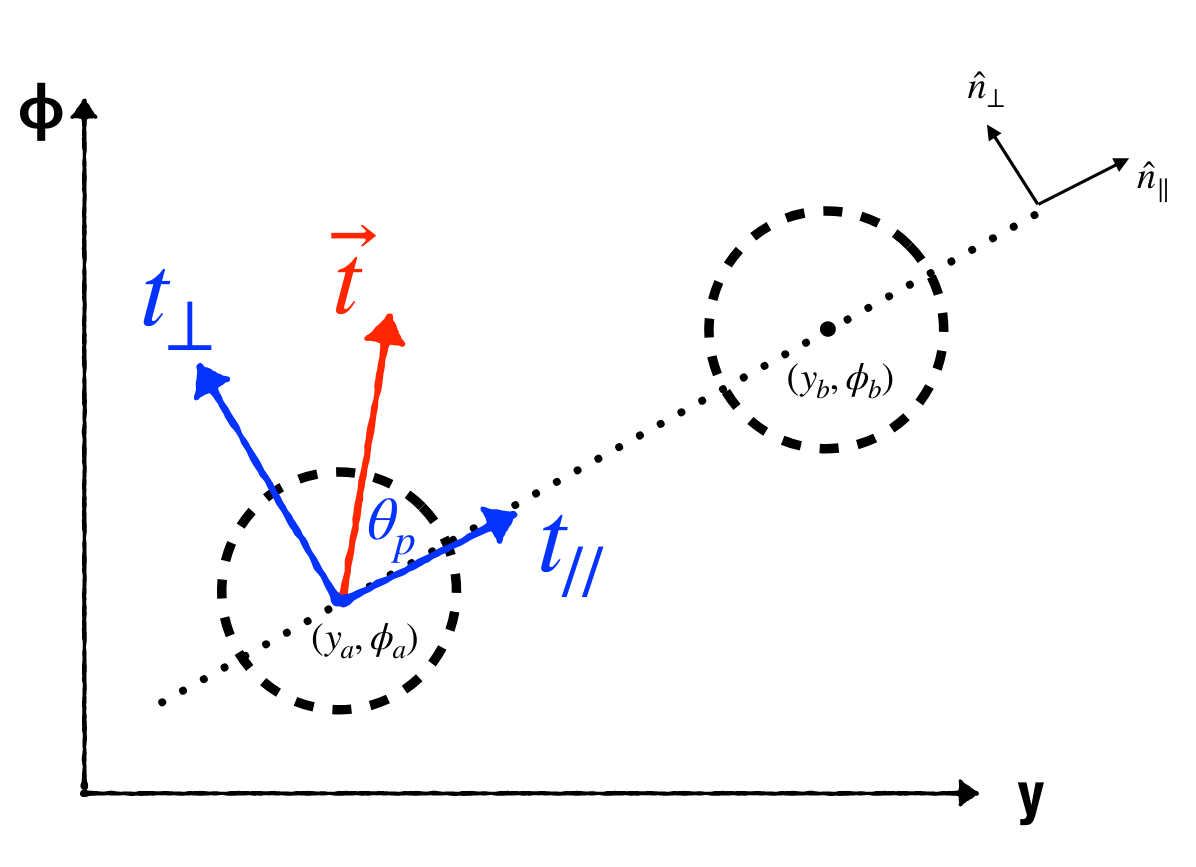
\includegraphics[scale=0.3]{ch4_images/pull_components}
\caption{A caption}
\label{Pull vector}
\end{figure}
The pull vector $\vec{t}$ relative to jet $J_a$ is defined as
\begin{equation}
\vec{t} = \frac{1}{p_{ta}} \sum_{i \in J_a}p_{ti}\vert \vec{r}_i \vert^2 \hat{r}_i
\end{equation}
where $p_{t_a}$ is the transverse momentum of the jet, and the sum runs over all the the jet constituents. $y$ and $\phi$ again represent rapidity and azimuthal angle, and $\vec{r}_i$ is the distance vector between the jet and its $i$-th constituent in the $y$-$\phi$ plane
\begin{equation}
\vec{r}_i = (y_i - y_a, \phi_i - \phi_a).
\end{equation}
In particular, we would like to consider the projections of $\vec{t}$ along two lines: one, generated by the unit vector which points from the center of $J_a$ to the center of $J_b$ of the two jets
\begin{equation}
\hat{n}_\parallel = \frac{1}{\sqrt{\Delta y^2 + \Delta \phi^2}}\left(\Delta y, \Delta \phi \right),
\end{equation}
and the other generated by the unit vector perpendicular to $\hat{n}_\parallel$
\begin{equation}
\hat{n}_\perp = \frac{1}{\sqrt{\Delta y^2 + \Delta \phi^2}}\left(-\Delta \phi, \Delta y \right),
\end{equation}
i.e.
\begin{gather}
t_\parallel = \vec{t}\cdot \hat{n}_\parallel \\
t_\perp = \vec{t}\cdot \hat{n}_\perp
\end{gather}
We would also like to consider $\theta_{p}$, known as the pull angle, defined as
\begin{equation}
\theta_p = \arccos \frac{t_\parallel}{\vert \vec{t} \vert}.
\end{equation} 

The pull vector is sensitive to the different color connections which are present in the decay of a color singlet and the decay of a color octet. An illustration of this feature is shown in Figure \ref{color connections}. Because of the different color connections, the radiation from jets originating from a singlet decay will tend to be emitted between the two jets, causing the pull vector of $J_a$ to point in the direction of $J_b$ and viceversa. In the octect case, the pull vectors will instead point in opposite \todo{(random?)} directions.
\begin{figure}[h]
\centering
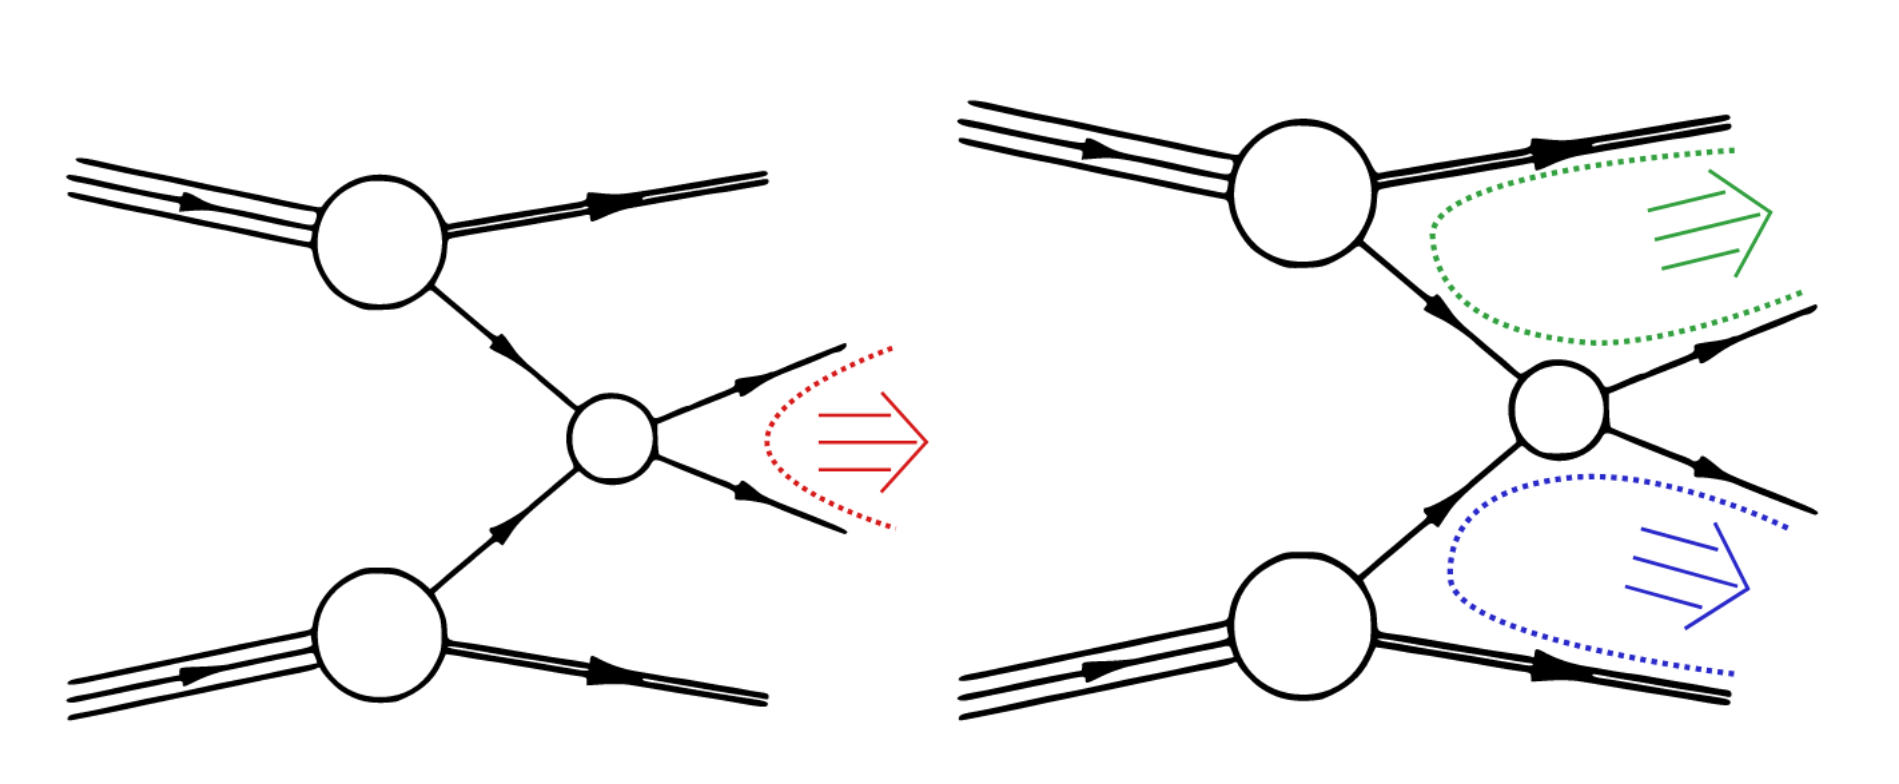
\includegraphics[scale=0.2]{ch4_images/color_configurations}
\caption{A representation of the color flow for the decay of a color singlet (left) vs. a color octect (right) at a collider experiment. In the case of a color singlet, the two colored particles stemming from the decay are color-connected only to each other, while for the case of an octect, the particles are color-connected to the rest of the proton, as it is from there that their color originates \cite{Gallicchio:2010sw}.}
\label{color connections}
\end{figure}
Of all the variables considered, the pull angle has been shown to be the most effective discriminator of the two different color configurations, \cite{Gallicchio:2010sw}. However, there was a noticeable mismatch between theoretical predictions for $\theta_p$ and experimental measurements \cite{Larkoski:2019urm}. 

The theoretical difficulties in calculating $\theta_p$ stem from the fact that it is not an IRC safe variable. However, $t_\parallel$ and $t_\perp$ \emph{are} IRC safe observables. 

Our method includes these two variables for this purpose. $\theta_p$ is also included since it can be measured at experiments, and its discrimination potential is still good. We consider the variables for both jets, thus 

\subsection{$D_2$}

To introduce the observable $D_2$, we must first familiarize the reader with energy correlator functions (ECF) \cite{Larkoski:2013eya}. These are a class of observables sensitive to jet substructure. Specifically, they are sensitive to a jet's \emph{prongedness}, or how many distinct subjets compose a given jet. This is particularly useful in the boosted regime, defined by $p_T \gg 1$, kinematics forces jets which would otherwise be separated to come together, as shown in Figure \ref{two pronged boost}. The $(N+1)$-point correlator is used to determine if a jet has $N$ prongs.

\begin{figure}
\centering
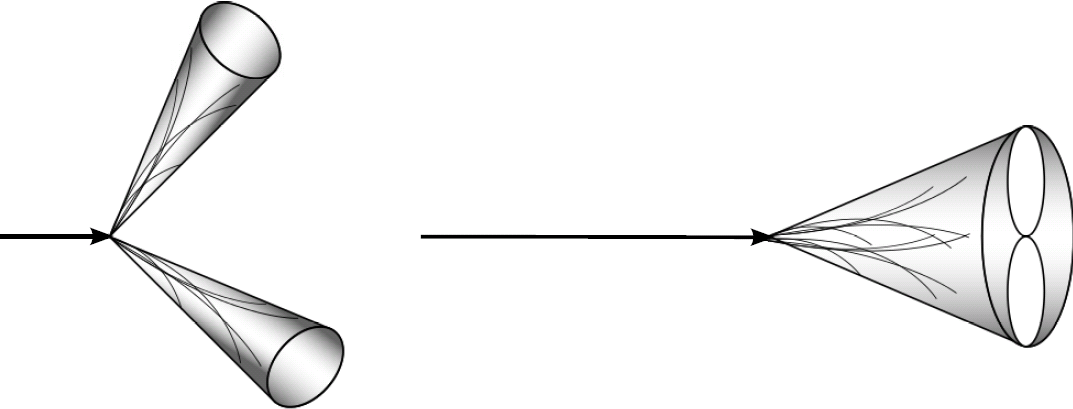
\includegraphics[scale=0.35]{ch4_images/two_prong}
\caption{An illustration of a 2-prong jet caused by boosted kinematics \todo{cite https://slidetodoc.com/download.php?id=7569163}.}
\label{two pronged boost}
\end{figure}

The definition of the N-point ECF is based on the  the $p_T$ and angular distance between the components of a jet:
\begin{equation}
ECF(N,\beta) = \sum_{i_1 < i_2 < \dots < i_N \in J} \left( \prod_{a = 1}^N p_{Ti_a} \right) \left(\prod_{b = 1}^{N-1} \prod_{c = b + 1}^N  R_{i_b i_c}\right)^\beta,
\label{ECF definition}
\end{equation}
where $\beta$ is an arbitrary parameter. If $\beta > 0$, the observable is IRC safe. 
For the sake of clarity, let us write out the first few ECFs:
\begin{gather*}
ECF(0, \beta) = 1\\
ECF(1, \beta) = \sum_{i\in J}p_{Ti} \\
ECF(2, \beta) = \sum_{i < j \in J} p_{Ti}p_{Tj} R_{ij}^\beta \\
ECF(3, \beta) = \sum_{i < j < k \in J} p_{Ti}p_{Tj}p_{Tk} \left(R_{ij}R_{ik}R_{jk}\right)^\beta.
\end{gather*}
There exists also a normalized $N$-point ECF, $e^{(\beta)}_N$, which differs from the definition (\ref{ECF definition}) by a factor proportional to the $p_T$ of the jet
\begin{equation}
e^{(\beta)}_N = \left(\frac{1}{p_{TJ}}\right)^N ECF(N,\beta)
\end{equation}

Clearly, $ECF(N,\beta) = 0$ when it is computed on a jet with fewer than $N$ constituents. In addition to this, $ECF(N+1, \beta)$ will be significantly smaller than $ECF(N,\beta)$ if calculated on a jet containing only $N$ subjets. This naturally leads to the consideration of the following ratio:
\begin{equation}
r_N^\beta = \frac{ECF(N+1,\beta)}{ECF(N,\beta)}.
\end{equation}
The ratio $r_N^\beta$ is useful to discriminate $N$-prong jets from $N+1$-prong jets. The $D_2$ variable \cite{Larkoski:2014gra} is a variation on this ratio, specified to the case of 1-prong and 2-prong jets, and calculated using the normalized ECFs
\begin{equation}
D_2(\beta) = \frac{e^{(\beta)}_3}{(e^{(\beta)}_2)^3}
\end{equation}
Due to the different color configurations, a large jet originating from the decay of a color singlet in the boosted regime will tend to exhibit a 2-prong substructure, and thus will tend to have a larger value of $D_2$. On the other hand, in the case of a color octect, the same decay will tend to have a 1-prong structure, leading to smaller values for the observable.

For the purpose of our study, we have chosen the value $\beta = 2$.

\subsection{Color Ring}
The final variable we have considered is known as the color ring \cite{Buckley:2020kdp}. To derive the observable, we must consider the boosted decay of a color singlet into two jets, which, at the parton level, correspond to (anti)quarks or gluons. We will consider the decay into two hard partons and the subsequent emission of a low-energy gluon.

The matrix element describing this transition is as follows:
\begin{equation}
\vert \mathcal{M}_S \vert^2 = -\mathbf{T}_\alpha \cdot \mathbf{T}_\beta 	\frac{n_a \cdot n_b}{(n_a \cdot k)(n_b \cdot k)}.
\end{equation}
In this expression, $n_a$ and $n_b$ are the light-like vectors parallel to the hard jets, $k$ is the impulse of the soft emission, and $\mathbf{T}_i$ is the color operator. The dependence on $\alpha_S$ has been neglected as it is not pertinent to the discussion. Latin indices are used to refer to kinematics while Greek indices refer to color.

We know that color must be conserved, as since we are dealing with a singlet decay, we must have
\begin{equation}
\mathbf{T}_\alpha + \mathbf{T}_\beta = 0.
\end{equation}
This necessarily implies that $\beta = \overline{\alpha}$, and so
\begin{equation}
-\mathbf{T}_\alpha \cdot \mathbf{T}_\beta = \mathbf{T}_\alpha^2 = C_S\mathbf{1}
\end{equation}
where $C_S$ is Casimir operator for either the fundamental or adjoint representation of $SU(3)$, depending on the decay, and we have explicitly written the identity matrix. 

Let us now consider the same matrix element for a background process, in which a color octect decays into two hard partons, with a subsequent soft emission in the boosted regime. Thanks to the boosted kinematics of the event, we can safely assume that the two hard partons are closer in angle to each other than to any other colored object, allowing for the factorization of the matrix element into two elements. The first describes the dipole formed by the hard partons and the emission of the soft radiation. The second contains additional contributions from the initial state of the event and from extra jets, if present. This term will again be neglected since it will lead to a constant. We can thus write
\begin{equation}
\vert \mathcal{M}_B \vert^2 = \sum_{\alpha, \beta} \left[ -\mathbf{T}_\alpha \cdot \mathbf{T}_\beta 	\frac{n_a \cdot n_b}{(n_a \cdot k)(n_b \cdot k)} - \mathbf{T}_\alpha \cdot \mathbf{T}_\gamma \frac{n_a \cdot \overline{n}}{(n_a \cdot k)(\overline{n} \cdot k)} - \mathbf{T}_\beta \cdot \mathbf{T}_\gamma 	\frac{n_b \cdot \overline{n}}{(n_b \cdot k)(\overline{n} \cdot k)} \right]
\label{bkg matrix element}
\end{equation}
where $\overline{n}$ is a light-like vector antiparallel to the system. $\overline{n}$ has overall color $\gamma$ which is fixed by the relation
\begin{equation}
\mathbf{T}_\alpha + \mathbf{T}_\beta + \mathbf{T}_\gamma = 0.
\end{equation}
We can use this to simplify the expression (\ref{bkg matrix element}), which becomes
\begin{equation}
\vert \mathcal{M}_B \vert^2 = \sum_{\alpha, \beta} \left[ -\mathbf{T}_\alpha \cdot \mathbf{T}_\beta 	\frac{n_a \cdot n_b}{(n_a \cdot k)(n_b \cdot k)} + (\mathbf{T}_\alpha^2 + \mathbf{T}_\alpha \cdot \mathbf{T}_\beta)\left(\frac{n_a \cdot \overline{n}}{(n_a \cdot k)(\overline{n} \cdot k)} + \frac{n_b \cdot \overline{n}}{(n_b \cdot k)(\overline{n} \cdot k)}\right) \right].
\end{equation}
The background matrix element has been written in terms of two color factors:
\begin{equation}
\begin{cases}
C_B = -\mathbf{T}_\alpha \cdot \mathbf{T}_\beta \\
\tilde{C}_B = \mathbf{T}_\alpha^2 + \mathbf{T}_\alpha \cdot \mathbf{T}_\beta.
\end{cases}
\end{equation}
Again, the exact color factor depends on the process considered. We are interested in $H\rightarrow b\overline{b}$ as our signal process, which fixes $C_S = C_F$ and $C_B = C_F - C_A/2$ and $\widetilde{C}_B = C_A/2$. A decay into gluons, e.g. $H\rightarrow gg$ would fix these constants differently.

It is a well-established fact that the optimal variable to discriminate these two configurations is monotonic in their ratio \cite{Neyman1992}. The ratio turns out to be
\begin{equation}
\frac{\vert \mathcal{M}_S \vert^2}{\vert \mathcal{M}_B \vert^2} \simeq \frac{(n_a \cdot \overline{n})(n_b \cdot k)}{(n_a \cdot n_b)(\overline{n} \cdot k)} + \frac{(n_b \cdot \overline{n})(n_a \cdot k)}{(n_a \cdot n_b)(\overline{n} \cdot k)}
\end{equation}
where we have left out the color factors as they are just constants. If we assume the collinear limit and utilize the small-angle approximation, this expression simplifies to 
\begin{equation}
\frac{\vert \mathcal{M}_S \vert^2}{\vert \mathcal{M}_B \vert^2} \simeq \frac{\theta_{ak}^2 + \theta_{bk}^2}{\theta_{ab}^2} \equiv \mathcal{O}.
\label{color ring}
\end{equation}
$\mathcal{O}$ is the definition of the jet color ring. This variable gets its name from its geometric interpretation, shown in Figure \ref{color ring geometry}. Radiation from color singlets will tend to fall between the two jets, leading to values of $\mathcal{O} < 1$, while in the case of color octects, we will tend to have $\mathcal{O} > 1$. 
\begin{figure}
\centering
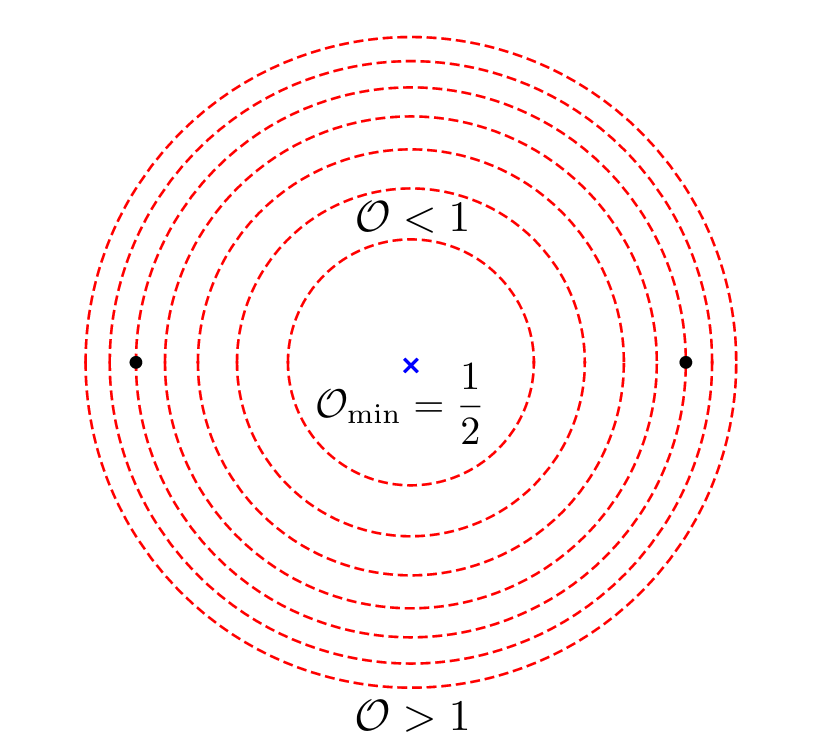
\includegraphics[scale=0.3]{ch4_images/cr}
\caption{A geometric interpretation of the color ring. The two black dots represent the two hard jets, and the contour passing through them has value $\mathcal{O} = 1$. Depending on the direction of $k$, the $\mathcal{O}$ can assume different values. If $k$ is collinear to either $a$ or $b$, $\mathcal{O}$ assumes its minimum value \cite{Buckley:2020kdp}.}
\label{color ring geometry}
\end{figure}

Unfortunately, without any sort of momentum-weighting, (\ref{color ring}) cannot be IRC safe. However, if we assume that the emission of the soft gluon leads to a distinct subjet within a larger jet, then IRC safety is recovered.

\section{The Simulation}

The aforementioned variables were produced via Monte Carlo simulation. Using \code{MadGraph5\_aMC} v2.8.3.2 \cite{Alwall:2014hca}, we generated two hard processes:
\begin{gather}
p p \rightarrow Z(\nu_\ell \overline{\nu}_\ell) H(b\overline{b}) \\
p p \rightarrow b\overline{b} \nu_\ell \overline{\nu}_\ell.
\end{gather}

The first process, hereby refered to as the signal, represents the most likely decay of the Higgs, a color singlet. The second process, or the background, contains all QCD diagrams which lead to the same final state as the signal. Figure \ref{zhbb + gbb feynman diagrams} shows the Feynman diagrams constituting signal and the background. The outputs of the parton-level simulations were saved as Les Houches Event Files \cite{Alwall:2006yp}.

\begin{figure}
\centering
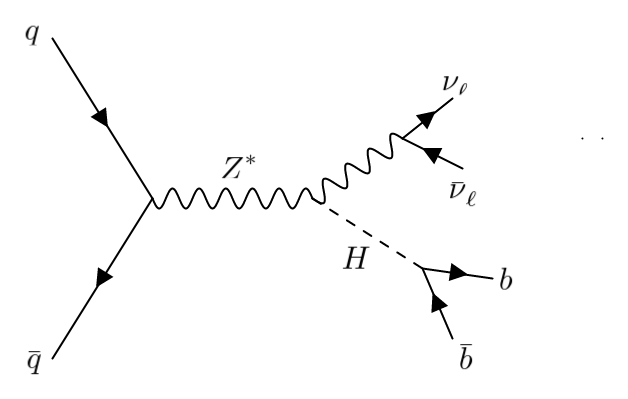
\includegraphics[scale=0.6]{ch4_images/zhbb}
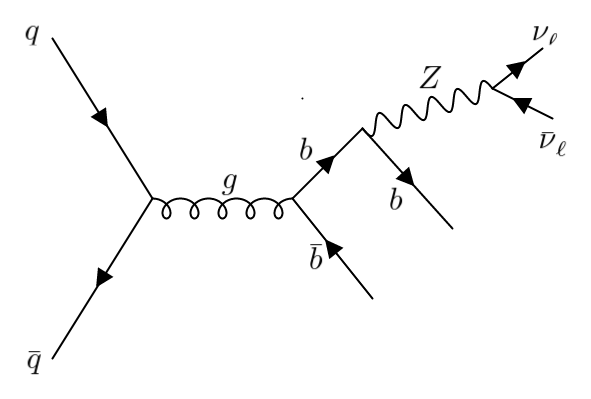
\includegraphics[scale=0.15]{ch4_images/gbb1}\\
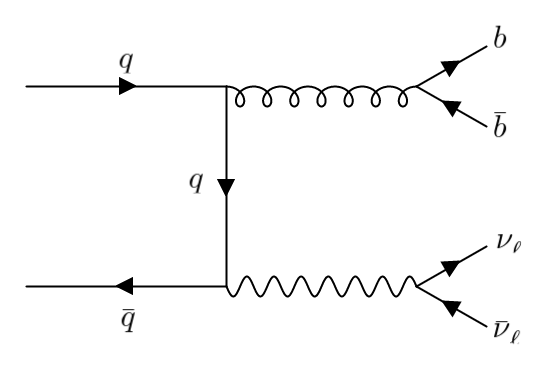
\includegraphics[scale=0.15]{ch4_images/gbb2}
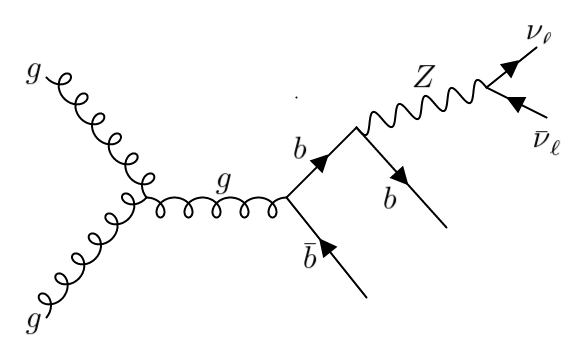
\includegraphics[scale=0.15]{ch4_images/gbb3}
\caption{The Feynman diagrams constituting the signal (upper left) and background. \todo{mettere immagine migliore}.}
\label{zhbb + gbb feynman diagrams}
\end{figure}

These hard processes were subsequently showered using two programs, \code{PYTHIA8} v8.305 \cite{Sjostrand:2014zea} and \code{Herwig} v7.2.2 \cite{B_hr_2008, Bellm:2015jjp} These programs simulate the perturbative evolution of the event (e.g. radiation) as well as hadronization to produce particle-level events. The simulations included both Multi Parton Interactions and underlying events. The output of the \code{PYTHIA8} shower was saved as a \code{HepMC3} file, and the output of the \code{Herwig} shower was saved as a \code{HepMC2} file \cite{BUCKLEY2021107310, Dobbs:2001ck}. \code{HepMC3} v3.2.2 and \code{HepMC2} v2.06.11 were used.

Since every program which simulates the parton shower necessarily includes its own systematic uncertainities, the shower in \code{Herwig} served as an independent check. We wanted to ensure that the results found were independent of the choice of parton shower, and thus that our results were reliable.

Finally, rather than simulating an entire detector, \code{Delphes} v3.5.0 was used to perform a fast detector simulation \cite{Ovyn:2009tx, deFavereau:2013fsa}. This allowed us to understand how our method would perform in reality without having to run the computationally expensive full simulation. From \code{Delphes}, we extracted both the Monte Carlo truth of the event, containing the particle level information, as well as the reconstructed events including the detector effects. 

The \code{Delphes} simulation was run using a version of the ATLAS card modified to fit our analysis standards. The output was stored as a \code{ROOT} file, and \code{ROOT} v6.22/06 was used \cite{fons_rademakers_2020_3895852}. 



\section{The Analysis}
Describe analysis steps, show plots of variables, describe statistics and most important cuts
\begin{enumerate}
\item Signal vs. Background true
\item Signal vs. Background reco
\item Signal Pythia vs. Signal Herwig (true)
\item Bkg Pythia vs. Bkg Herwig (true)
\end{enumerate}

\section{Machine Learning}
Describe architectures

\section{Results}
ROC curves, various cuts and their influences

\section{Further Studies}
Mass bias \\
show that method works also for $Z\rightarrow b\overline{b}$?

\section{Conclusions}
Discuss integration with Lund Plane \\
Measurement and training of real data \\
Addition to Xbb tagger

%Descrivere la simulazione (aggiungere diagrammi di feynman)
%Descrivere l'analisi + mostrare plot (entro mercoledì)
%Machine Learning algorithms (descrivere architetture)
%Results (ROC curves)
%Further Studies - Mass debiasing, Z->bb
%Conclusion Future prospects, Lund plane, ecc. 
\end{document}